\documentclass[aspectratio=169]{beamer}

\setbeamertemplate{footline}[frame number]

\usepackage{hyperref}
\usepackage{caption}
\captionsetup[figure]{labelformat=empty}

\title{Exploratory analysis of Recurrent deforestation warnings in São Félix do 
Xingu - Brazilian Amazon}

\author{Alber Sanchez\\alber.ipia@inpe.br}
\institute{
    
\includegraphics[width=4cm,keepaspectratio]{./logos/trees-color-h_2.png}
    
\includegraphics[width=1.8cm,keepaspectratio]{./logos/logoinpe-azul-menor.png} \\
    TreesLab\\Instituto Nacional de Pesquisas Espaciais - INPE\\Brazil
}
\date{\today}

\begin{document}

%---- 01 ----
\frame{\titlepage}

%---- 02 ----
\begin{frame}
    \frametitle{Introduction}
    \begin{itemize}
        \item Deforestation by successive degradation remains a challenging 
            question in the scientific literature.
        \item We think a potential answer to this question could be found in 
            DETER's warning.
        \item This answer could play an important role, for example, for 
            improving the national estimation of greenhouse gases.
        \item We used DETER data from 2016 to 2021 of São Félix de Xingu, Pará, 
            Brazil.
        \item São Félix de Xingu is among the towns with the highest 
            deforestation rates according to PRODES.
    \end{itemize}
\end{frame}

%---- 03 ----
\begin{frame}
    \frametitle{What is DETER?}
    \begin{itemize}
        \item DETER is a GIS which produces a fast assessment of deforestation 
            and forest degradation in the Brazilian 
            Amazon~\cite{shimabukuro2006}.
        \item DETER is an important tool for environmental protection and  
            effective law enforcement.
        \item DETER employs Linear Mixture Models of CBERS imagery and  human
            experts to deter and issue warnings of deforested (or degraded) 
            areas larger than 3 ha~\cite{dealmeida2022}.
        \item Annually, DETER takes from PRODES the current forested area, 
            stating anew issuing warnings.
    \end{itemize}
\end{frame}

%---- 04 ----
\begin{frame}
    \frametitle{São Félix do Xingu, Pará, Brazil}
    \begin{figure}[h] 
        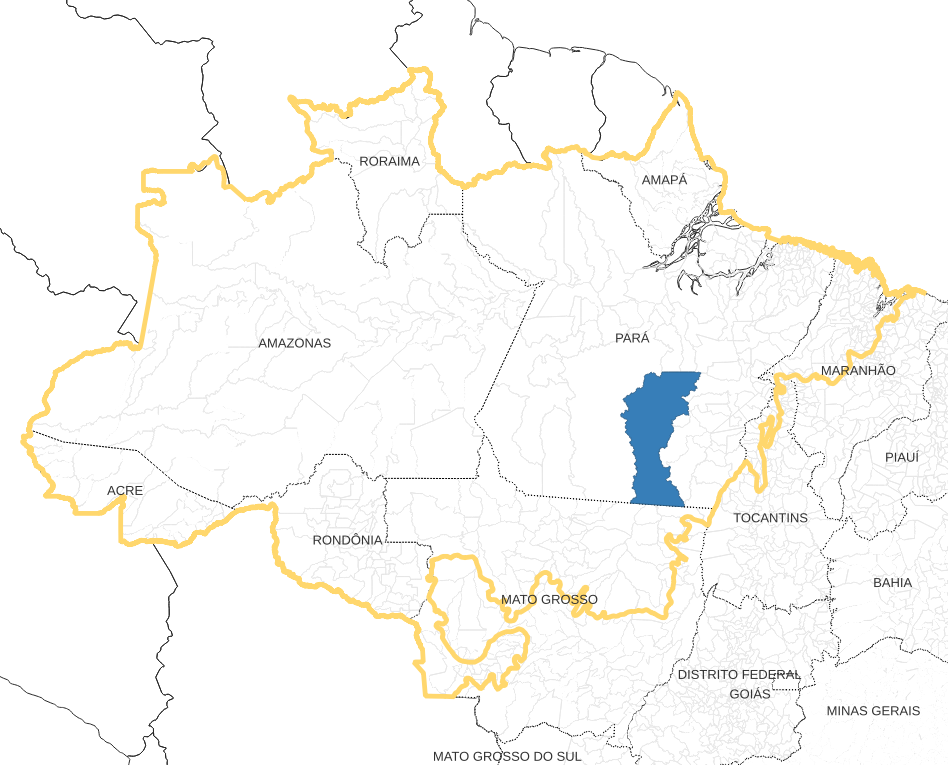
\includegraphics[width=0.65\linewidth]
        {./figures/sao_felix_do_xingu.png}
        \label{fig:sao_felix_do_xingu}
    \end{figure}
\end{frame}

%---- 05 ----
\begin{frame}
    \frametitle{DETER warnings in São Félix do Xingu}
    \begin{figure}[h] 
        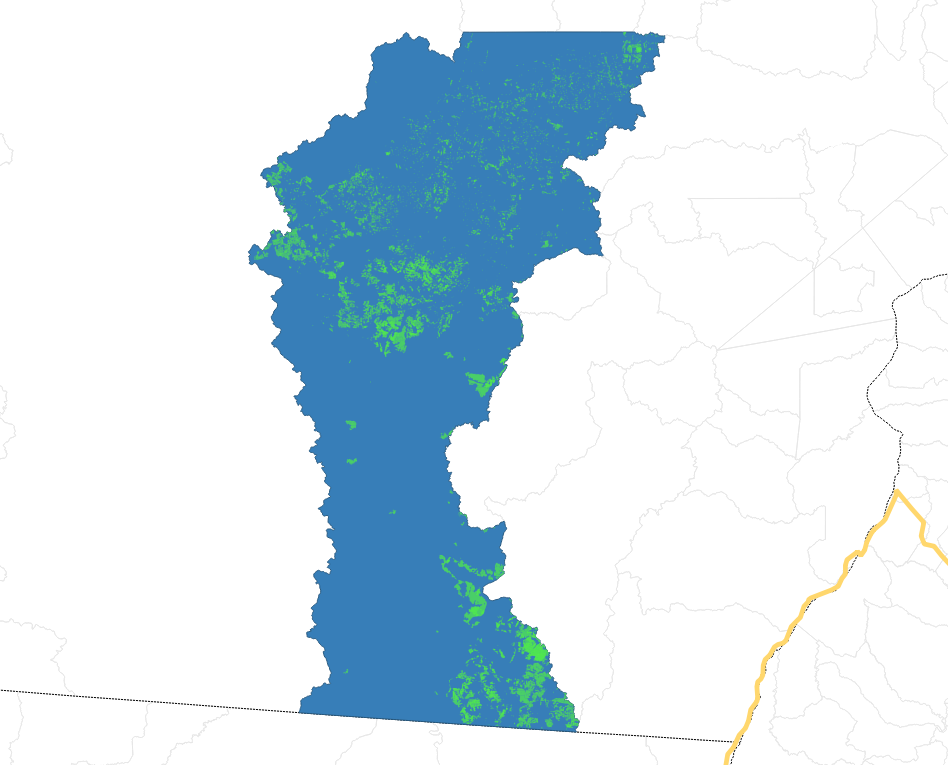
\includegraphics[width=0.65\linewidth]
        {./figures/deter_sao_felix_do_xingu.png}
        \label{fig:sao_felix_do_xingu}
    \end{figure}
\end{frame}

%---- 06 ----
\begin{frame}
    \frametitle{Area of DETER warnings in SFX}
    \begin{figure}[h] 
        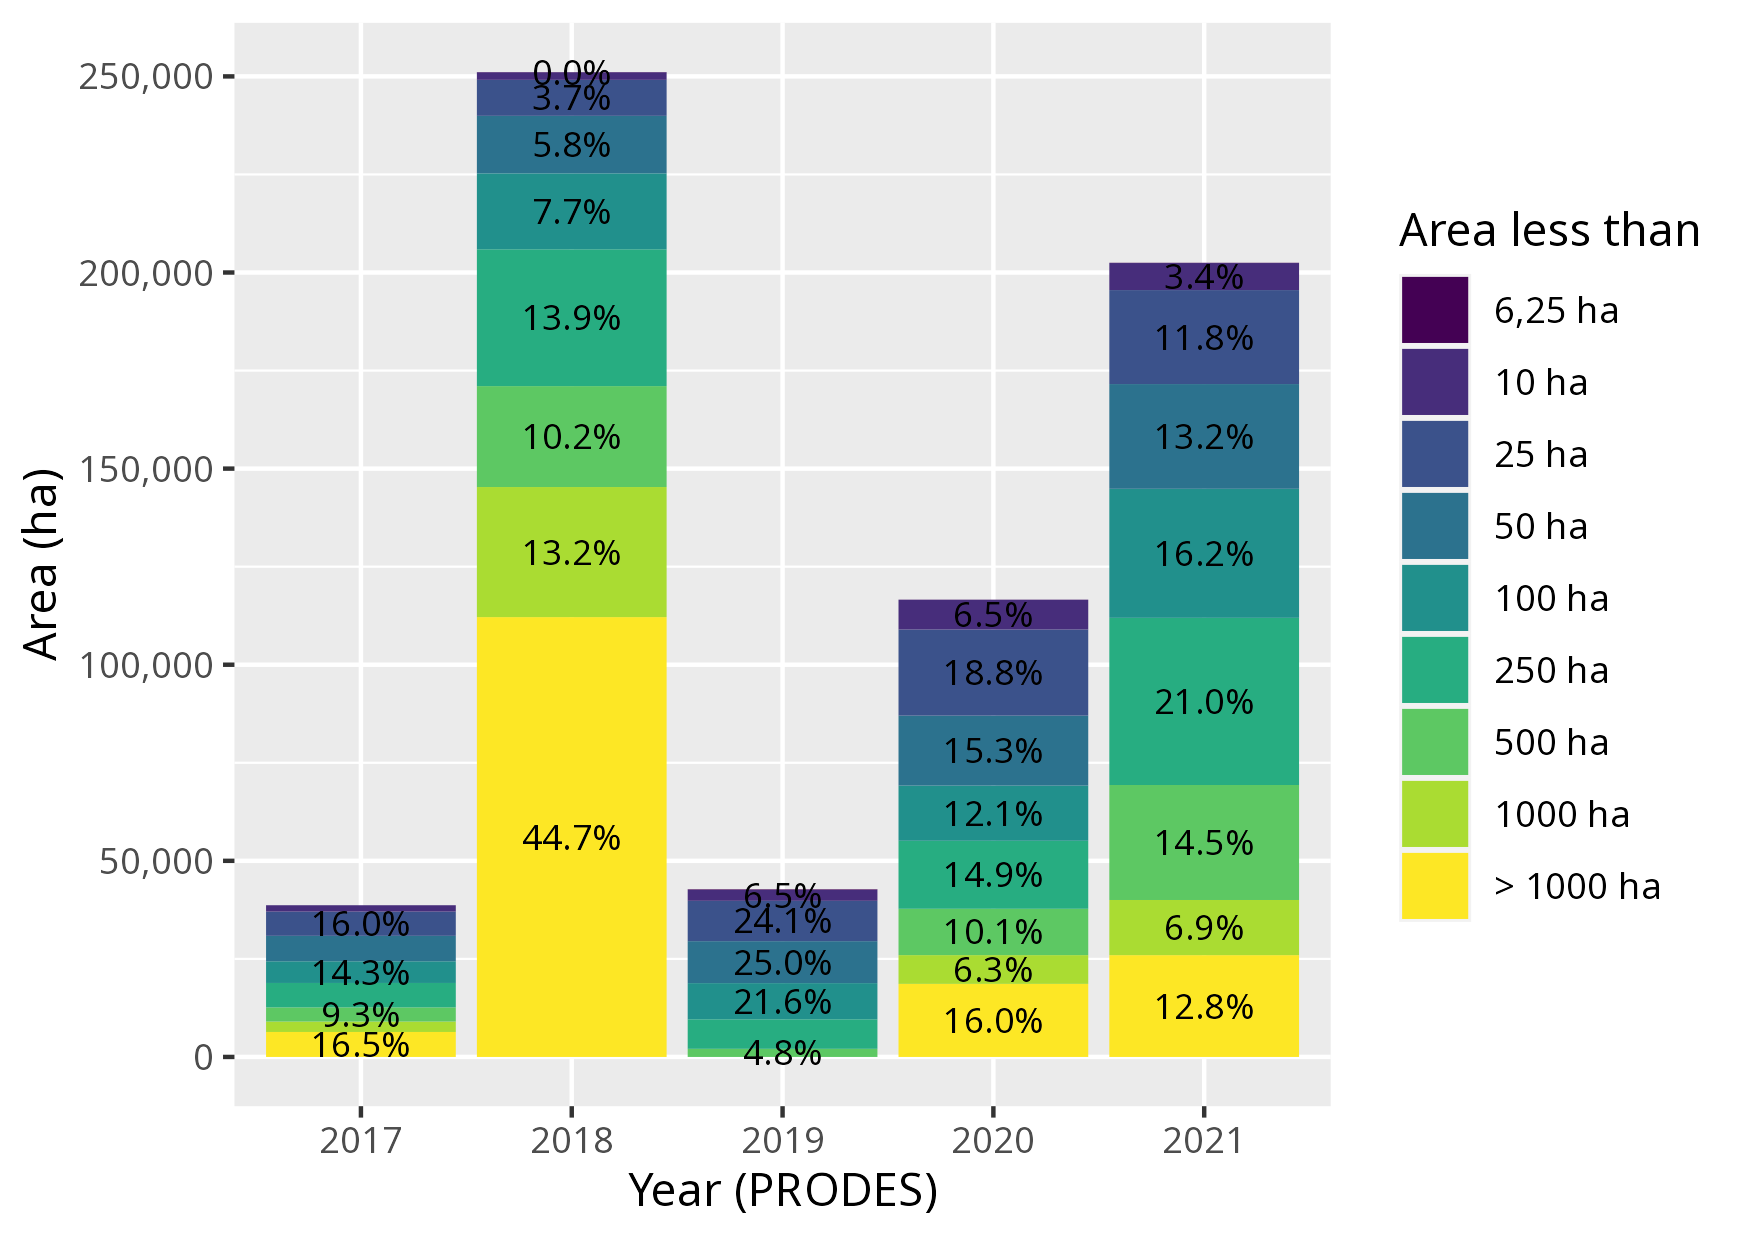
\includegraphics[width=0.65\linewidth]
        {./figures/deter_warnings_area_size.png}
        \caption{Note the increasing trend and its area distribution.}
        \label{fig:deter_warnings_area}
    \end{figure}
\end{frame}

%---- 07 ----
\begin{frame}
    \frametitle{Number of DETER warnings in SFX}
    \begin{figure}[h] 
        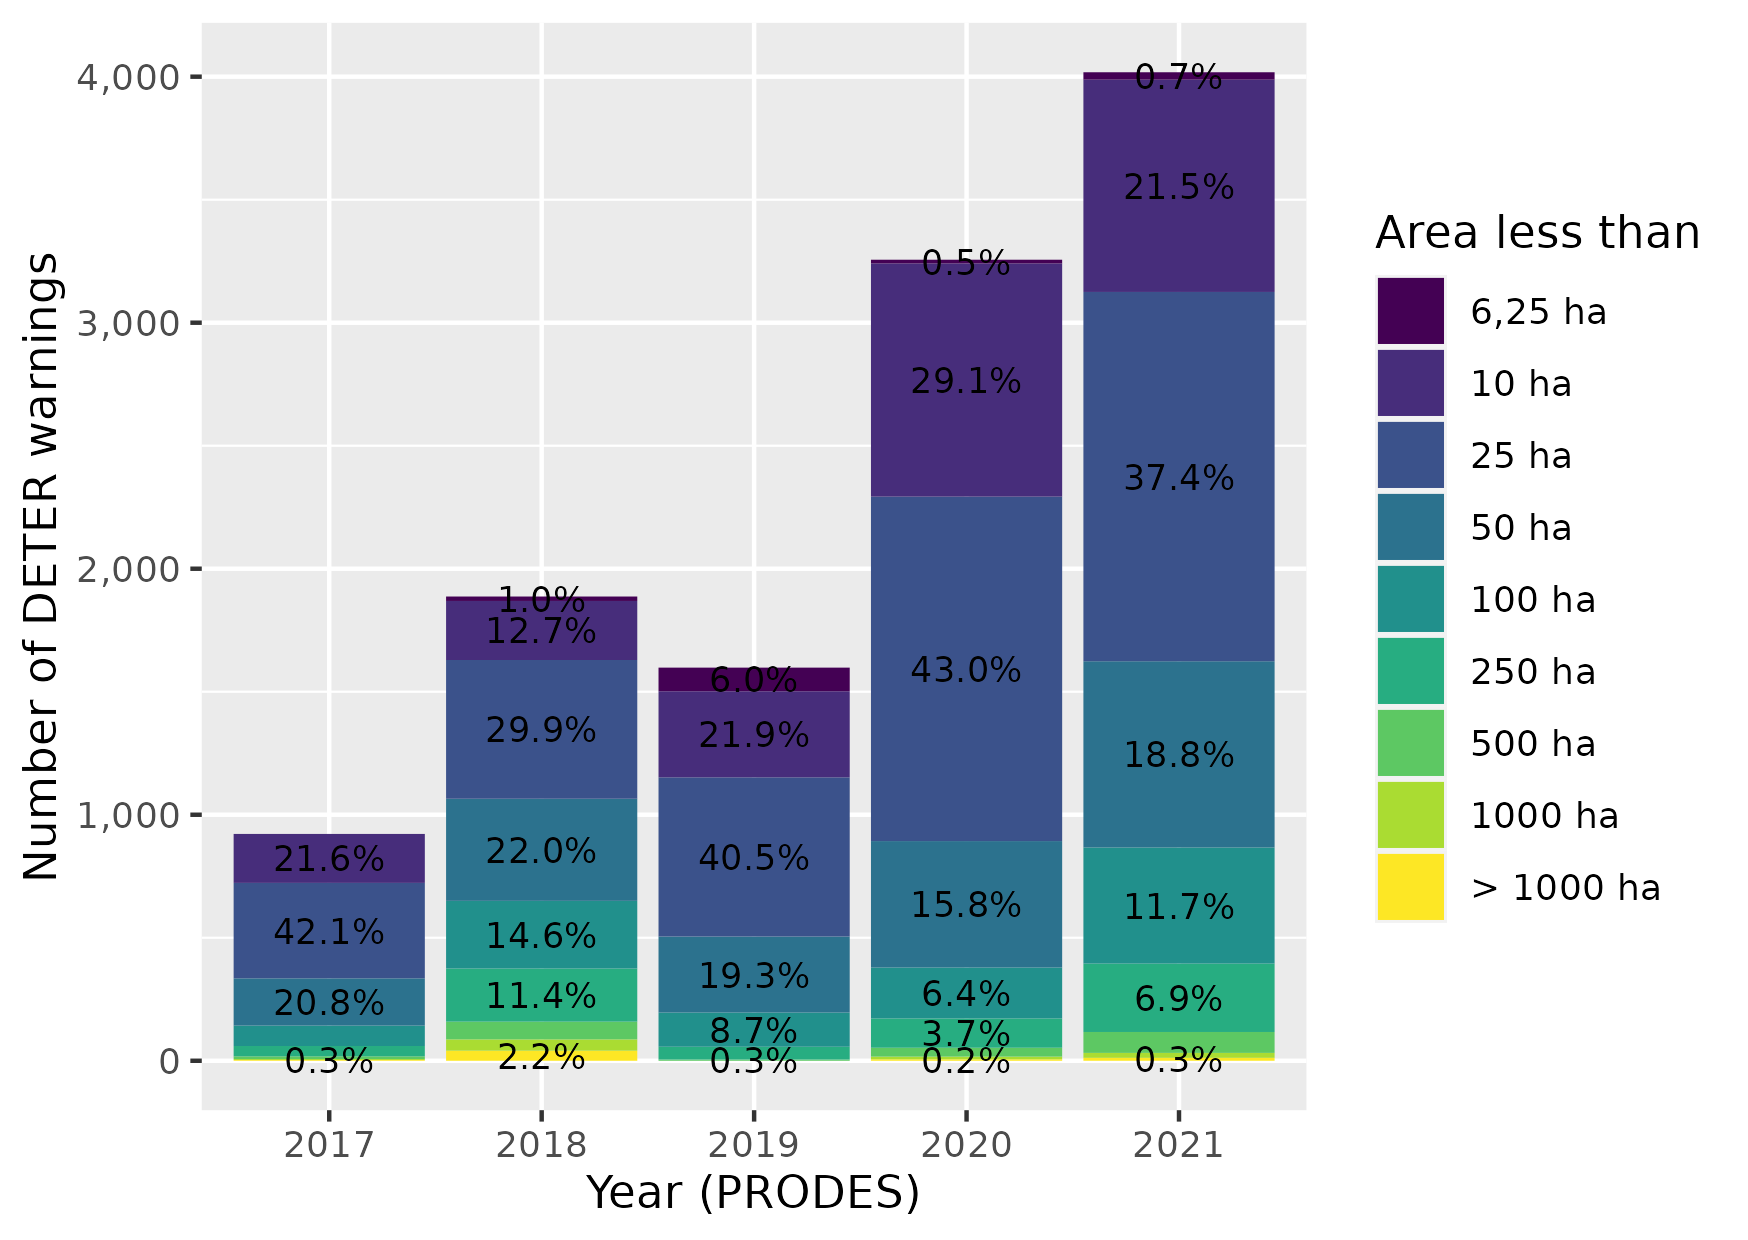
\includegraphics[width=0.65\linewidth]
        {./figures/deter_warnings_size.png}
        \caption{Note the increasing trend and the small peak in 2018.}
        \label{fig:deter_warnings_number}
    \end{figure}
\end{frame}

%---- 08 ----
\begin{frame}
    \frametitle{Periodicity of DETER warnings in SFX}
    \begin{figure}[h] 
        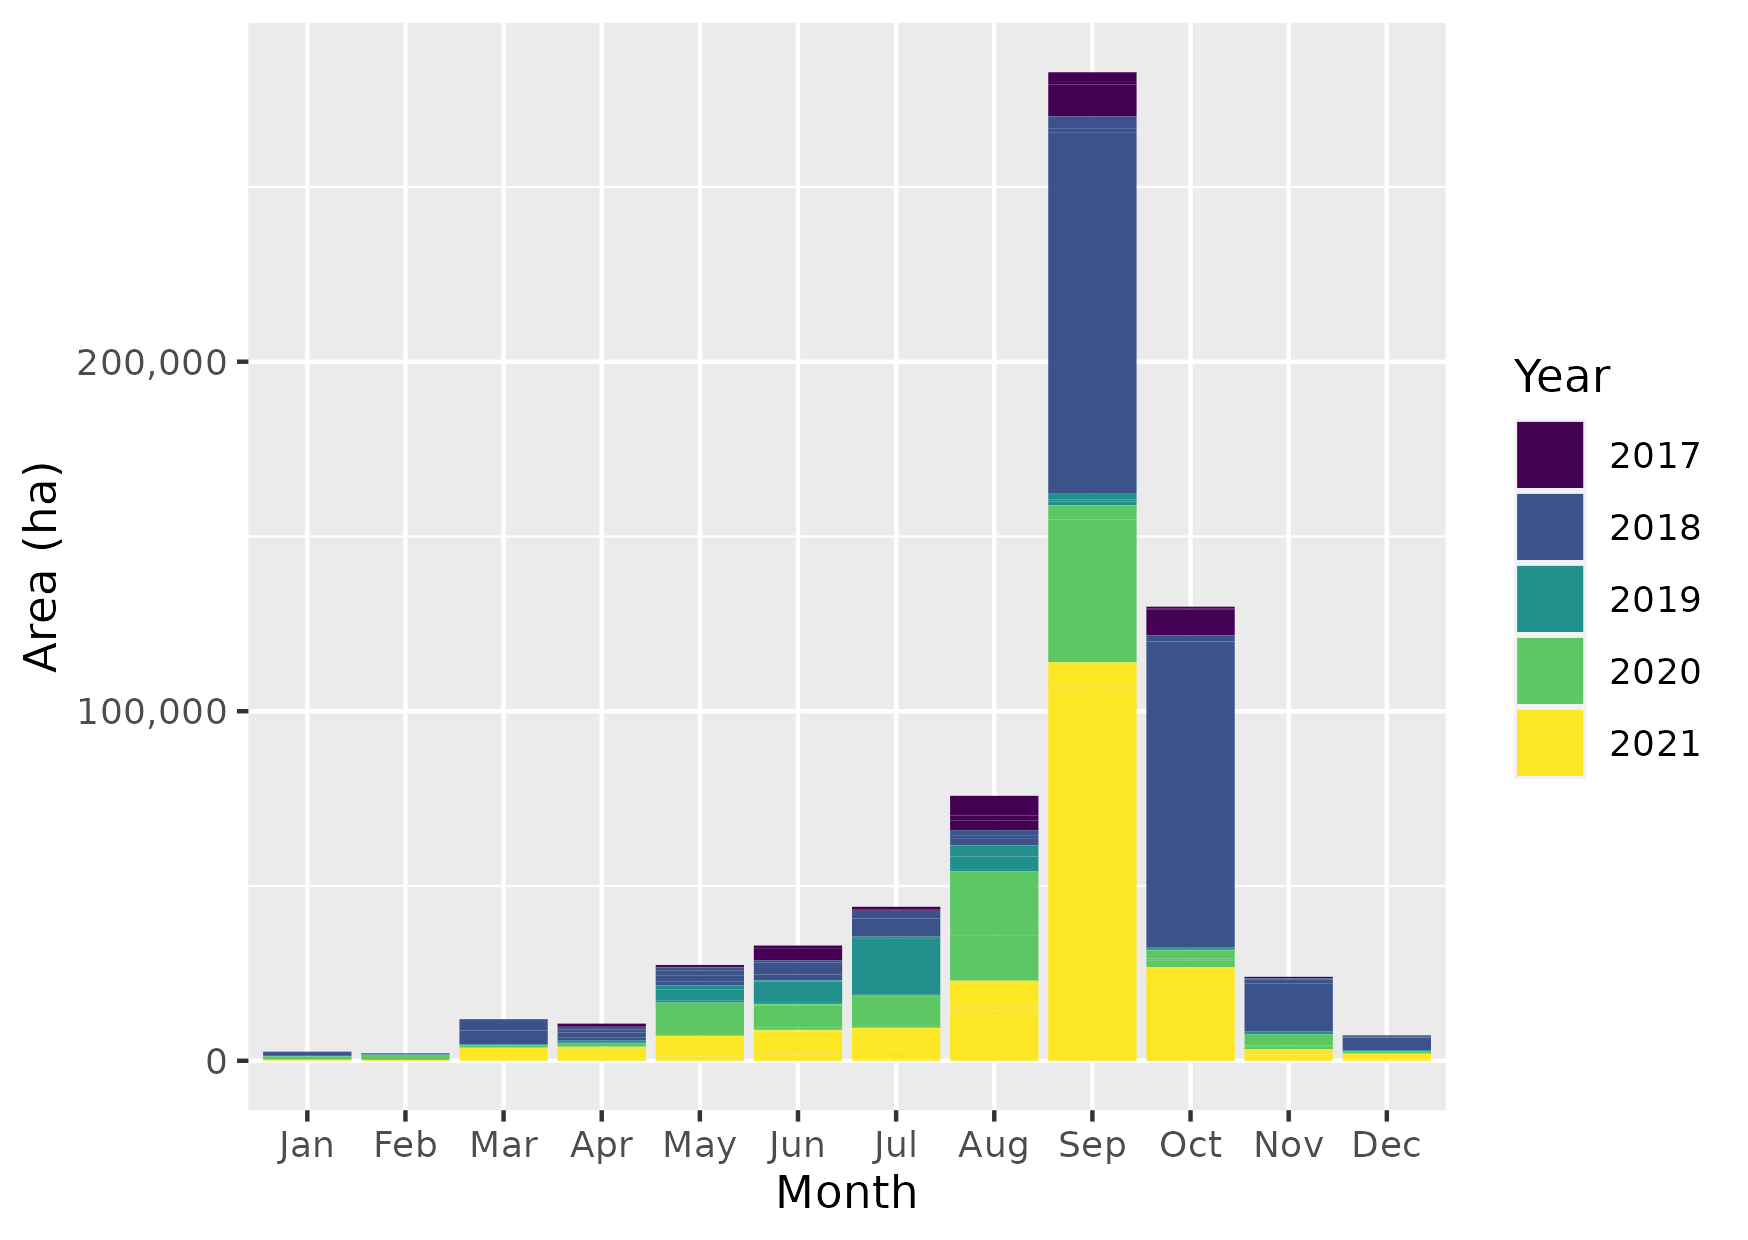
\includegraphics[width=0.65\linewidth]
        {./figures/deter_warnings_size_month.png}
        \caption{Note Sep-Oct 2018 and Aug-Sep 2020 }
        \label{fig:deter_warnings_periodicity}
    \end{figure}
\end{frame}

%---- 09 ----
\begin{frame}
    \frametitle{DETER warnings and time}
    \begin{itemize}
        \item The spatial properties of DETER warning areas are inconsistent 
            along time (shape, size, area, position).
    \end{itemize}
\end{frame}

%---- 10 ----
\begin{frame}
    \frametitle{Warning subareas are inconsistent along time}
    \begin{figure}[h] 
        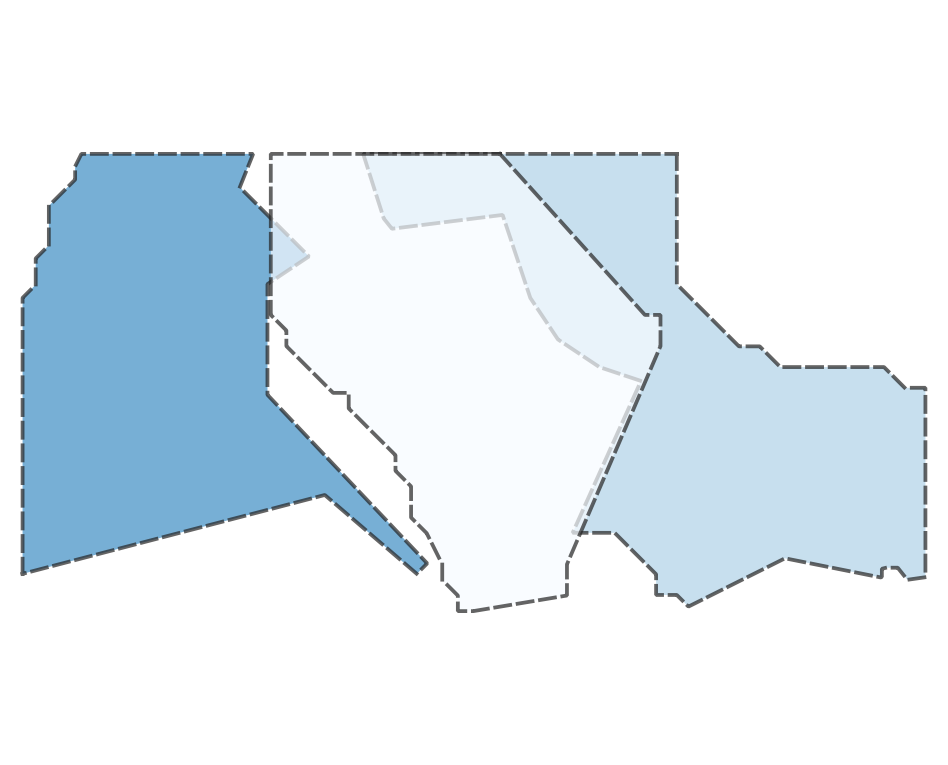
\includegraphics[width=0.60\linewidth]
        {./figures/sample_deter_warnings.png}
        \label{fig:deter_subareas}
        \caption{Note how DETER warnings overlap differently with time.}
    \end{figure}
\end{frame}

%---- 11 ----
\begin{frame}
    \frametitle{DETER warnings subareas}
    \begin{itemize}
        \item The spatial properties of DETER warning areas are inconsistent 
            along time (shape, size, area, position).
        \item DETER subareas maintain their spatial properties along time.
    \end{itemize}
\end{frame}

%---- 12 ----
\begin{frame}
    \frametitle{DETER warning subareas}
    \begin{figure}[h] 
        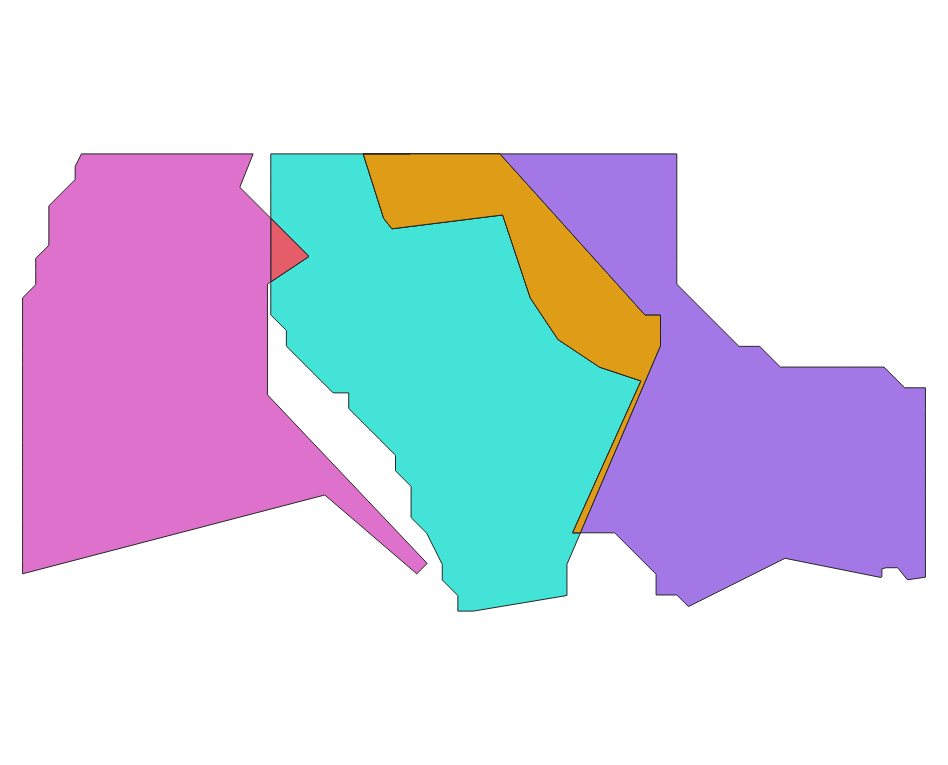
\includegraphics[width=0.60\linewidth]
        {./figures/sample_deter_subareas.png}
        \caption{Note how 3 DETER warnings produce 7 subareas!}
        \label{fig:deter_subareas}
    \end{figure}
\end{frame}

%---- 13 ----
\begin{frame}
    \frametitle{Subareas of recurrent warnings}
    \begin{figure}[h] 
        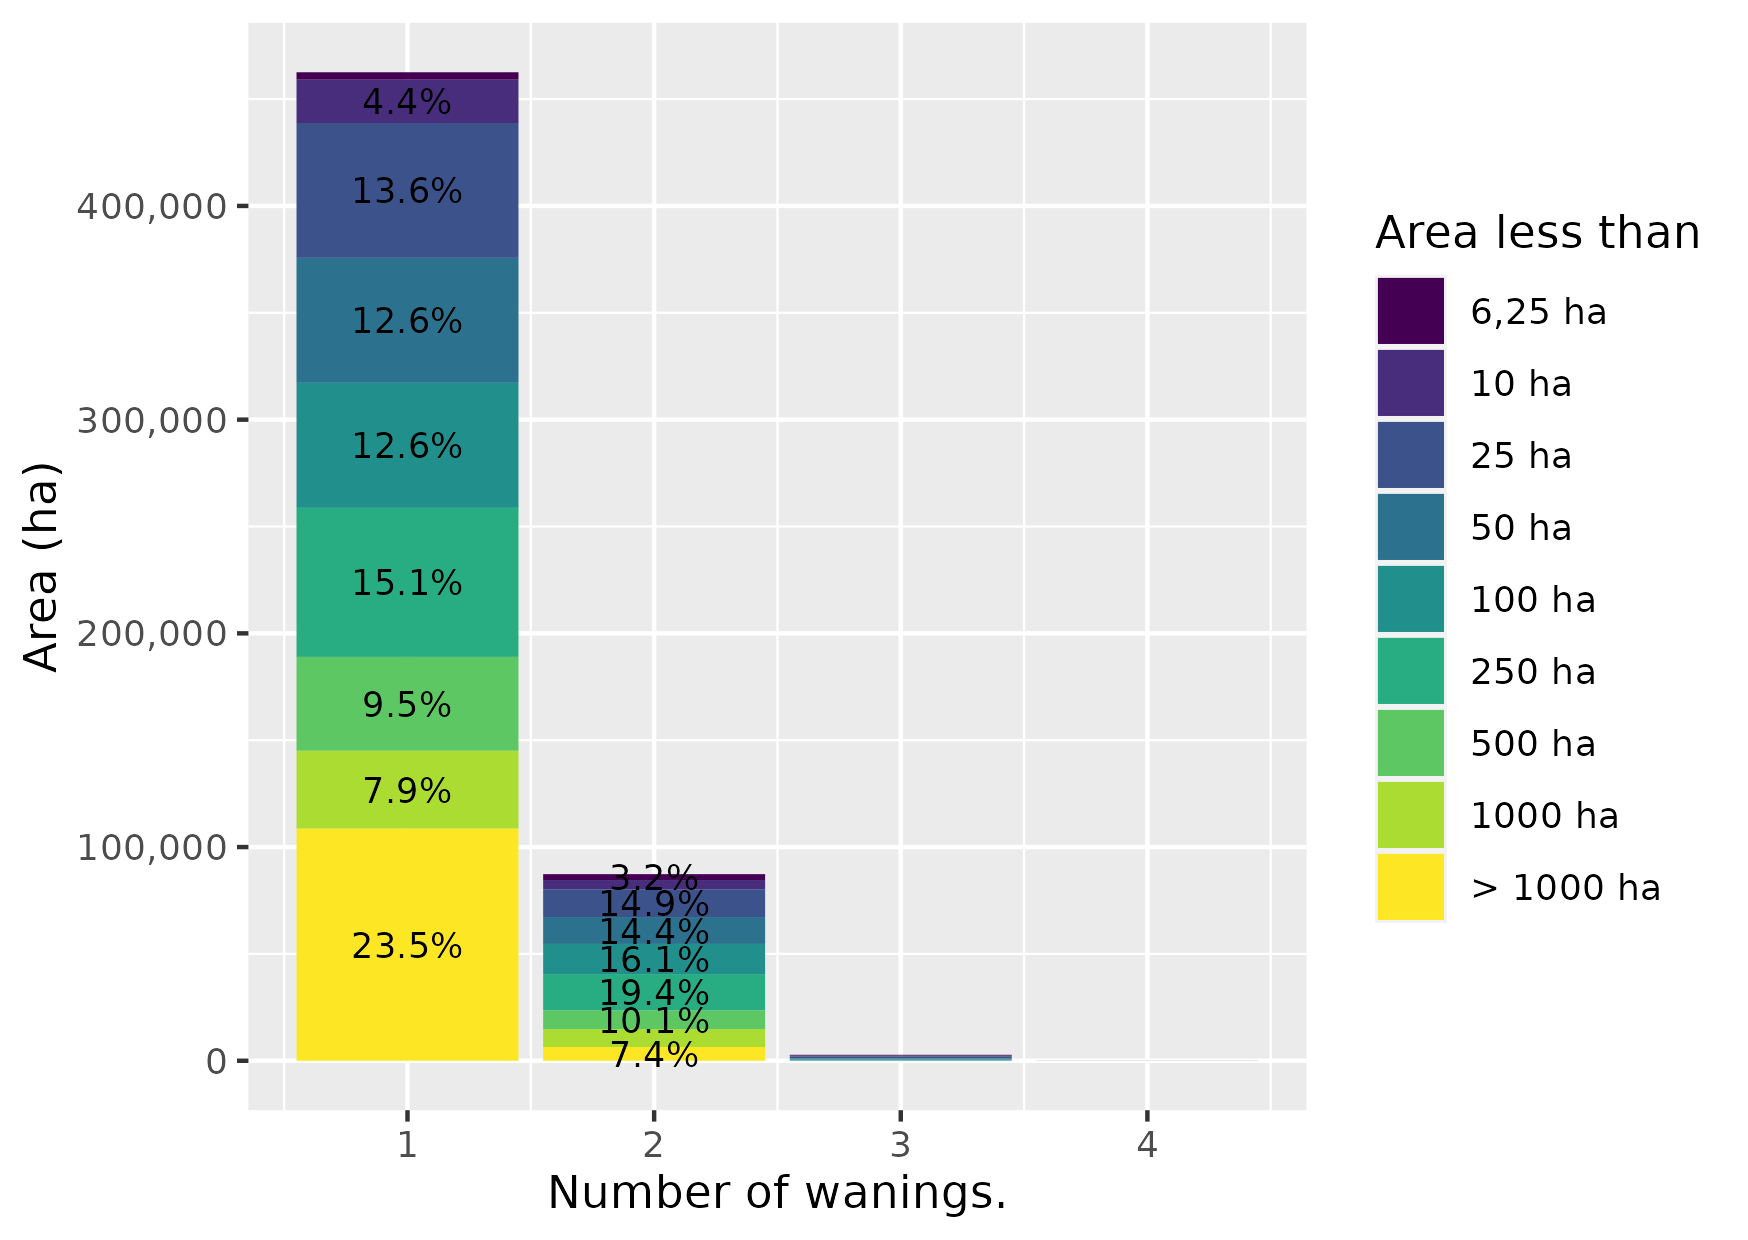
\includegraphics[width=0.65\linewidth] 
        {./figures/plot_area_by_warnings.png}
        \caption{Most subareas are issued a single warning.}
        \label{fig:deter_warning_recurrency}
    \end{figure}
\end{frame}

%---- 14 ----
\begin{frame}
    \frametitle{Days between first and last warnings}
    \begin{figure}[h] 
        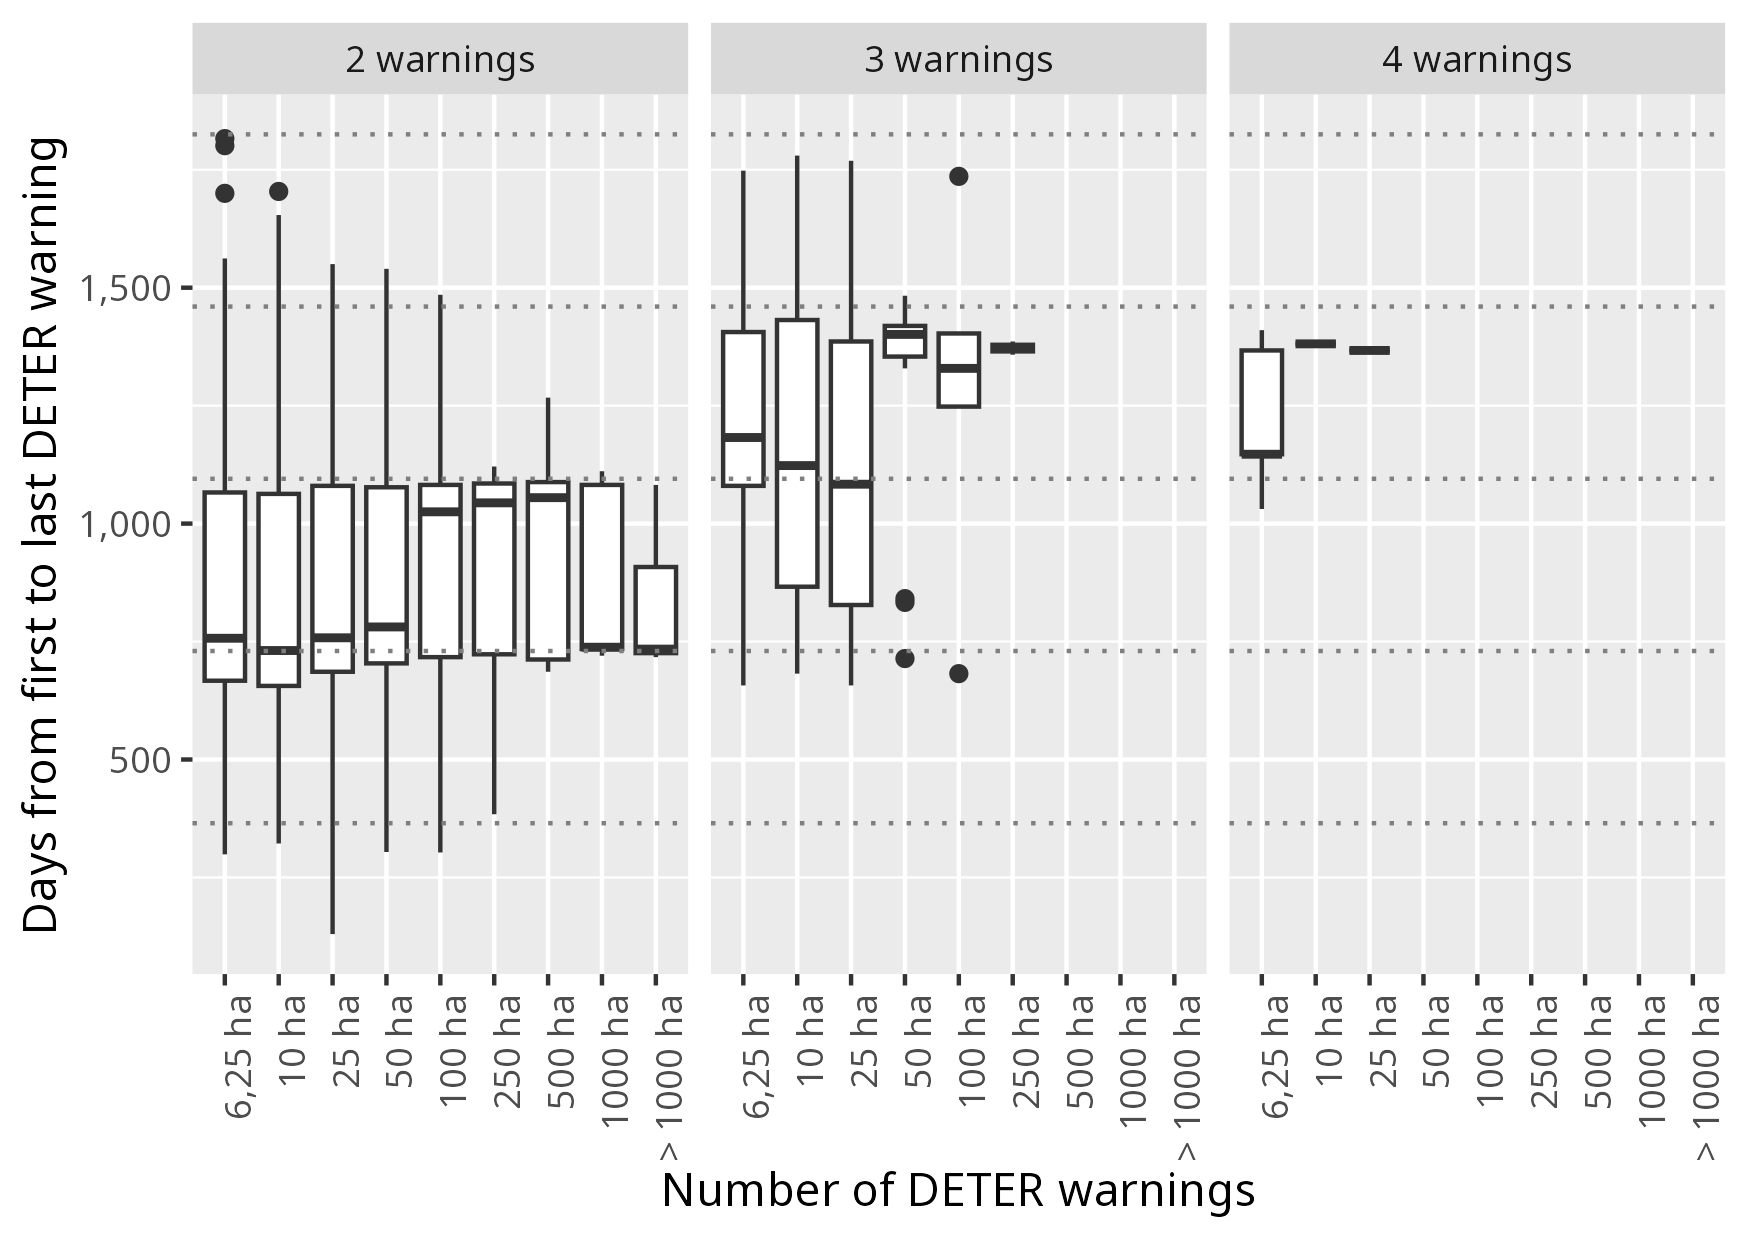
\includegraphics[width=0.65\linewidth]
        {./figures/plot_days_first_to_last.png}
        \caption{The mean lag between 2 and 3 warnings is one year.}
        % NOTE: Each Box plot shows the median; 
        %       the first and third quartiles (hinges); 
        %       1.5 times the inter-quartile range from the hinges; 
        %       and the outliers.
        \label{fig:deter_warning_first_to_last}
    \end{figure}
\end{frame}

%---- 15 ----
\begin{frame}
    \frametitle{Reproducibility - DETER processing}
    \begin{figure}[h] 
        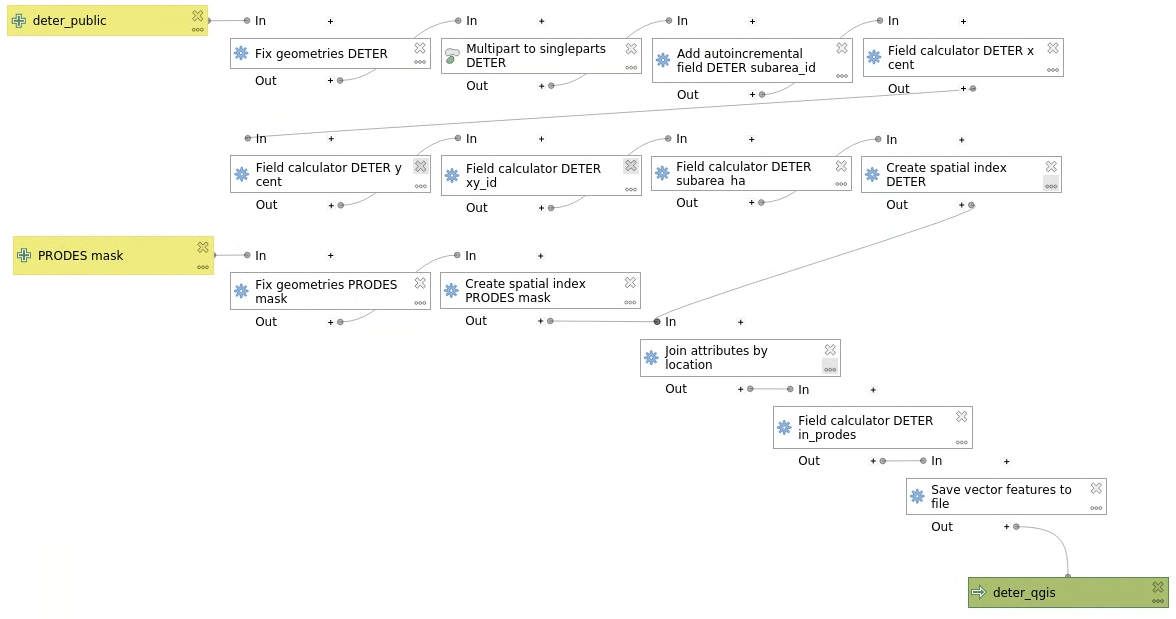
\includegraphics[width=0.95\linewidth] 
        {./figures/deter_processing.png}
        \caption{DETER data preprocessiing before analysis.}
        \label{fig:deter_processing}
    \end{figure}
\end{frame}

%---- 16 ----
\begin{frame}
    \frametitle{Final remarks}
    \begin{itemize}
        \item The analysis of DETER warning subareas along time could improve 
            the characterization of forest degradation along time.
        \item Potential applications of our work are:
            \begin{itemize}
                \item Improve estimation of emissions of greenhouse gases, i.e.
                    our data could help avoiding double counting.
                \item Identify spatio-temporal areas which could help training 
                    Machine-Learning algorithms for automatic indentification 
                    of forest degradation.
            \end{itemize}
        \item Code available at 
            \url{https://github.com/albhasan/treesburnareas}
    \end{itemize}
\end{frame}

%---- 17 ----
\begin{frame}[allowframebreaks]
    \frametitle{References}
    \bibliographystyle{amsalpha}
    \bibliography{07_SBSR.bib}
\end{frame}

\end{document}
